\documentclass[12pt, a4paper, oneside]{report}

\usepackage[utf8]{inputenc}
\usepackage[T1]{fontenc}
\usepackage[polish]{babel}
\usepackage{setspace}
\usepackage{titlesec}
\usepackage[pdftex]{graphicx}     
\usepackage{float}


\titleformat{\section}[block]{\Large\bfseries}{}{1em}{}
\usepackage[font={small, it}]{caption}


\title{\Huge \textbf{Znajdowanie potrzeb}\\
       \large \textbf{Raport z zadania}\\\,\\
       \Large Komunikacja człowiek-komputer 2019}
\date{\,\\7 listopada 2019}
\author{Jakub Grobelny\\ Jakub Remiszewski\\ Kacper Bukowiec}

\setstretch{1.4}

\begin{document}

\begin{titlepage}
    \maketitle
    \thispagestyle{empty}
\end{titlepage}

\renewcommand*\thesubsection{\arabic{section}}

\section*{Opis problemu}

Kolej jest bardzo popularnym środkiem transportu, szczególnie wśród studentów,
ale często można spotkać się z opiniami, że proces internetowego zakupu biletu 
na pociągi PKP Intercity nie jest szczególnie przyjemnym doświadczeniem. 
Postanowiliśmy przyjrzeć się temu zagadnieniu i zbadać, jak różne osoby radzą 
sobie z obsługą strony internetowej PKP Intercity.

\section*{Opis badania}

Każdą osobę biorącą udział w badaniu poprosiliśmy o
próbę kupienia biletu z Wrocławia do Szczecina na stronie internetowej
PKP Intercity (dokładniej o dotarcie do momentu wyboru sposobu
płatności). Obserwowaliśmy cały proces a następnie zadaliśmy
badanym kilka pytań o to jakie były ich subiektywne odczucia na temat
strony internetowej.

\section*{Osoby badane}

\begin{itemize}
    \item \textbf{osoba A}: Kobieta w wieku 22 lat. Studentka 4 roku 
    architektury na Politechnice Wrocławskiej. Styczność z komputerami ma 
    regularnie.
    \item \textbf{osoba B}: Pani Wiesława, lat 83, emerytowana sklepowa 
    sprzedawczyni.
    Dotychczasowo kupowała bilety w “okienku” i nigdy wcześniej nie kupowała
    biletów przez internet. Jako osoba niezaznajomiona z nowymi technologiami
    miewa problemy w poruszaniu się na skomplikowanych stronach internetowych. 
    \item \textbf{osoba C}: Pan Jakub, pracownik Instytutu Informatyki 
    Uniwersytetu Wrocławskiego.
\end{itemize}

\section*{Przebieg badania}

\begin{itemize}
    \item \textbf{A:} Badana przeszła przez cały proces zakupu bez żadnych 
    problemów, gdyż dobrze znała całą procedurę. 
    \item \textbf{B:} Pani Wiesława wyglądała na wyraźnie zagubioną po 
    posadzeniu przed komputerem. Używanie myszki sprawiało jej problem i miała 
    trudności z wycelowaniem w odpowiednie miejsce. Szybko zmieniające się 
    reklamy na stronie głównej rozpraszały ją (o czym wspomniała) ale w miarę 
    sprawnie znalazła pola do wpisywania stacji. Nie zauważyła jednak, że datę 
    można zmienić strzałkami oraz przez ikonkę kalendarza więc wpisała datę 
    ręcznie. Gdy przeszła do kolejnej strony kursor myszy wylądował na polu 
    gdzie wybiera się pociąg, więc gdy chciała użyć kółka myszy aby przejść w 
    dół, lista pociągów przesunęła się horyzontalnie. Pani Wiesława wybrała z 
    listy ulgę „Bilet dla Seniora” ale niestety nie zauważyła, że domyślnie 
    wybrany jest też jeden bilet według taryfy normalnej. Swoją pomyłkę
    zauważyła dopiero na następnym ekranie, gdy cena była wyższa niż być powinna.
    \item \textbf{C:}  Przy pierwszej próbie wyszukania połączenia w 
    przeglądarce Firefox nastąpił błąd. Choć nie było otwartej dodatkowej karty 
    ani dodatkowego okna, trzeba było zmienić przeglądarkę. Wyszukanie 
    połączenia i wybranie konkretnej trasy przebiegło bez problemów. Przy 
    wybraniu biletu z ulgą nastąpił problem z wybraniem odpowiedniej zniżki, 
    lista była nieczytelna, źle zorganizowana. Kolejne kroki Pan Jakub 
    przeszedł bez problemu.
\end{itemize}

\begin{figure}[]
    \centering
    
\includegraphics[scale=0.30]{./pani-wieslawa.png}
    \caption{Pani Wiesława po zobaczeniu strony głównej PKP Intercity.}
    \label{}
\end{figure}




\section*{Ankieta i odpowiedzi badanych}

Po wykonaniu czynności, zadaliśmy badanym poniższe pytania (część z nich 
było pytaniami zamkniętymi, część otwartymi). Pod każdym pytaniem znajdują
się odpowiedzi kolejnych osób.

\begin{itemize}
    \item\textbf{Czy uważasz, że strona PKP Intercity jest czytelna i 
    przejrzysta?}
    \begin{itemize}
        \item \textbf{A:} raczej nieczytelna
        \item \textbf{B:} bardzo nieczytelna
        \item \textbf{C:} średnio
    \end{itemize}

    \item\textbf{Czy miałeś kiedykolwiek problemy z kupnem biletu?}
    \begin{itemize}
        \item \textbf{A:} \textit{,,tak, chciałam kupić bilet dla dwóch osób 
        towarzyszących ale miejsca brakowało miejsc i informacja o tym pojawiła 
        się dopiero na ostatniej stronie.''}
        \item \textbf{B:} \textit{,,tylko teraz, wcześniej nie kupowałam 
        biletów przez internet''}
        \item \textbf{C:} \textit{,,Kupiłem bilet intercity pierwszy raz po 
        pięcioletniej przerwie''}
    \end{itemize}

    \item\textbf{W skali 1-10 jak oceniasz poziom trudności zakupu biletu.?}
    \begin{itemize}
        \item \textbf{A:} 7/10
        \item \textbf{B:} 9/10
        \item \textbf{C:} 5/10
    \end{itemize}

    \item\textbf{Jak często kupujesz bilety kolejowe?}
    \begin{itemize}
        \item \textbf{A:} \textit{,,Średnio raz lub dwa razy w tygodniu.''}
        \item \textbf{B:} \textit{,,Kilka razy w roku''}
        \item \textbf{C:} \textit{,,Bardzo rzadko w Polsce, częściej za 
        granicą.''}
    \end{itemize}

    \item\textbf{Czy poruszanie się po stronie PKP Intercity sprawia Ci 
    niekiedy problem?}
    \begin{itemize}
        \item \textbf{A:} \textit{,,Tak, bo nie jest wygodna w obsłudze.''}
        \item \textbf{B:} \textit{,,Tak, jest na niej dużo rozpraszających 
        rzeczy''}
        \item \textbf{C:} \textit{,,Tak, niekiedy.''}
    \end{itemize}

    \item\textbf{Czy twoim zdanie sposób wybierania rodzaju biletu jest dobrze 
    zaprojektowany?}
    \begin{itemize}
        \item \textbf{A:} \textit{,,Jest w miarę OK.''}
        \item \textbf{B:} \textit{,,Chyba nie, bo łatwo jest coś źle 
        zaznaczyć''}
        \item \textbf{C:} \textit{,,Nie.''}
    \end{itemize}

    \item\textbf{Czy możliwość wyszukiwania i kupowania dwóch biletów 
    jednocześnie jest dla ciebie istotna?}
    \begin{itemize}
        \item \textbf{A:} zdecydowanie tak
        \item \textbf{B:} raczej nie
        \item \textbf{C:} zdecydowanie tak
    \end{itemize}

    \item\textbf{Co byś zmienił/zmieniła w stronie PKP Intercity?}
    \begin{itemize}
        \item \textbf{A:} \textit{,,Dodałabym pokazywanie wolnych miejsc w 
        wagonie.''}
        \item \textbf{B:} \textit{,,Większe litery.''}
        \item \textbf{C:} \textit{,,Możliwość podejrzenia poprzedich kroków 
        oraz podsumowania wybranych biletów. Możliwość otwierania strony w 
        wielu kartach.''}
    \end{itemize}
\end{itemize}

\section*{Potrzeby}

Na podstawie obserwacji badanych oraz własnych doświadczeń wytypowaliśmy 
dziesięć potrzeb, które należy spełnić implementując system elektronicznego 
zakupu biletów kolejowych:

\begin{enumerate}
    \item Możliwość wyszukiwania wielu połączeń w jednym momencie.
    \item Możliwie wiele form płatności przy zakupie biletu.
    \item Czytelna strona główna, na której głównym elementem jest wyszukiwarka połączeń a nie reklamy.
    \item Wizualizacja wolnych i zajętych miejsc w wagonie.
    \item Możliwie krótki proces zakupu biletu.
    \item Niepowodzenie na którymkolwiek etapie nie powinno wymagać rozpoczęcia całego procesu od nowa.
    \item Wyświetlanie ceny od razu w momencie wyboru rodzaju biletu.
    \item Wyświetlanie informacji o średnim opóźnieniu wybranego pociągu.
    \item Interaktywny czat z konsultantem.
    \item Możliwość szybkiego wybrania często używanego połączenia dla zarejestrowanych użytkowników.
\end{enumerate}

\begin{figure}[H]
    \centering
    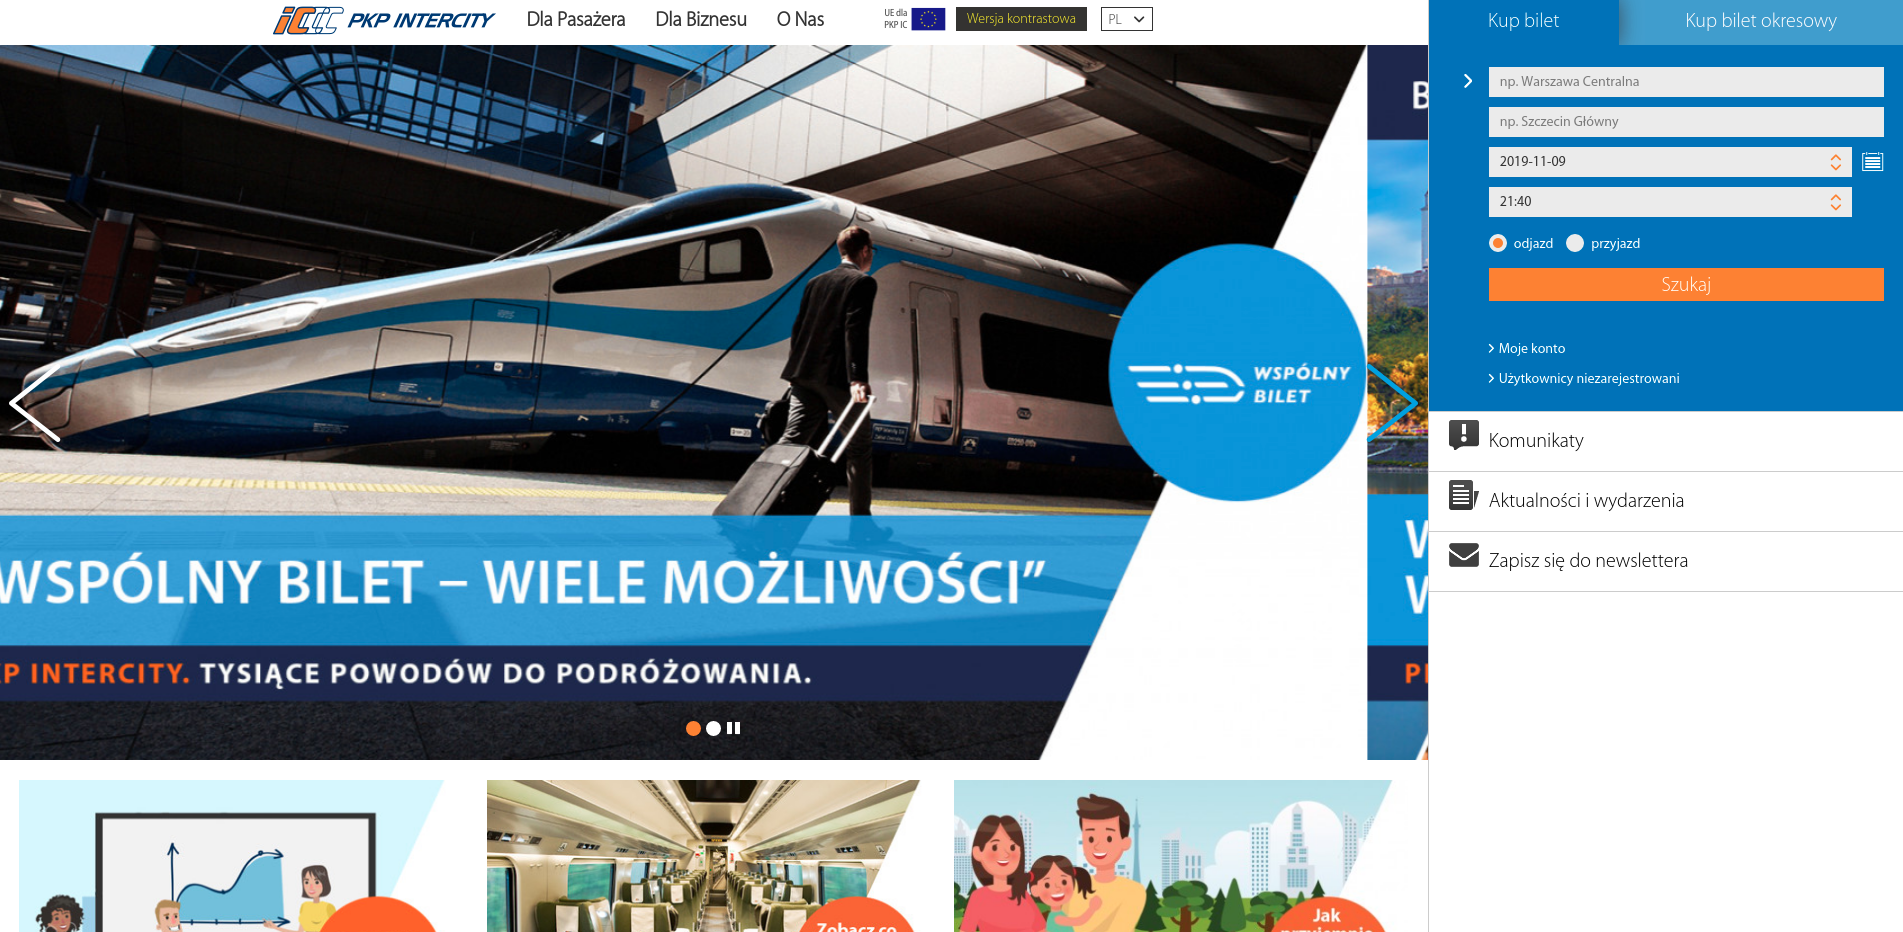
\includegraphics[scale=0.18]{./pkp-main.png}
    \caption{Zaśmiecona reklamami strona główna.}
    \label{}
\end{figure}


\section*{Propozycje ulepszeń}

Proponujemy również następujące możliwości ulepszenia istniejącej strony:

\begin{enumerate}
    \item Umożliwienie istnienia więcej niż jednej sesji dla danego użytkownika 
    co pozwoli na jednoczesne wyszukiwanie biletów w obie strony. Obecnie nie 
    jest możliwe sprawdzanie kilku opcji, gdyż otworzenie strony w nowej karcie 
    kończy się komunikatem o tym, że praca została już rozpoczęta w innej 
    karcie lub oknie przeglądarki.
    \item Dodanie nowych form płatności (na przykład PayPal, paysafecard, 
    Bitcoin). Różni ludzie mają różne preferencje co do sposobu płatności a 
    aktualnie wybór jest bardzo ograniczony.
    \item Umieszczenie wyszukiwarki połączeń w centralnej części strony tak aby 
    reklamy nie odwracały od niej uwagi co może być problematyczne dla osób, 
    które nie są przyzwyczajone do szumu informacyjnego panującego w 
    internecie. Strona główna jest zaśmiecona reklamami PKP Intercity co 
    zmniejsza jej czytelność.
    \item Cały proces zakupu biletu powinen odbywać się na jednej stronie a w 
    razie niepowodzenia na którymkolwiek etapie proces powinien zostać 
    wznowiony w miejscu, w którym wystąpił problem. Cofnięcie się do 
    poprzedniego etapu nie powinno powodować zrestartowania całej
    czynności. Wystarczy drobny bląd żeby zostać zmuszonym do rozpoczęcia całego
    czasochłonnego procesu od nowa co jest bardzo frustrujące.
    \item Wizualizacja rozkładu miejsc w wybranym wagonie wraz z informacją o 
    tym czy miejsca są zajęte czy wolne. Dodanie możliwości wyboru miejsca poprzez graficzny interfejs. W aktualnej wersji strony nie ma opcji 
    dowiedzenia się jaki jest rozkład  miejsc i wybiera się je w ciemno.
\end{enumerate}

\begin{figure}[H]
    \centering
    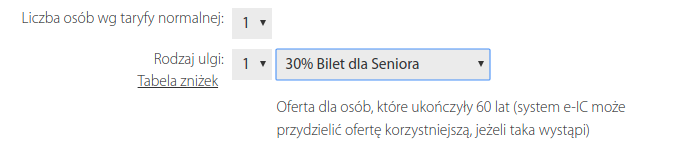
\includegraphics[scale=0.55]{./pkp-ticket-type.png}
    \caption{Źle zaprojektowany interfejs do wyboru rodzaju biletu.}
    \label{}
\end{figure}

\end{document}















